\documentclass{article}
% =======PACKAGES=======
% FORMATTING
\usepackage{amssymb}
\usepackage{amsmath}
\usepackage{breqn}
\usepackage{graphics}
\usepackage{graphicx, wrapfig}
\usepackage{latexsym}
\usepackage{setspace}
\usepackage{hyperref}

\hypersetup{
    colorlinks=true,
    linkcolor=blue,
    filecolor=magenta,      
    urlcolor=cyan,
    pdftitle={Traveling Salesman Problem Approaches},
    pdfpagemode=FullScreen,
}

%\usepackage{algorithm2e}

\usepackage[margin=0.625in]{geometry}
\usepackage{parskip, setspace}
\setstretch{1.15}
\renewcommand{\arraystretch}{1.25}
% TYPESETTING - MATH
\usepackage{amsmath, amsfonts}
\usepackage[ruled, linesnumbered, noend]{algorithm2e}
\RestyleAlgo{ruled}
% RICH
\usepackage{caption}

% BIBLIOGRAPHY
\usepackage{natbib}
\bibliographystyle{unsrt}

% =======TITLE=======
\title{\vspace*{-0.625in}CS 565: Scientific Computing \\ Project 2: The Traveling Salesman Problem using Ant Colony Optimization and Discrete Gravitational Search\vspace*{-0.25in}}
\author{Nathan Chapman, Hunter Lawrence, Andrew Struthers}
\date{\today}

\begin{document}

\maketitle
\tableofcontents
\pagebreak
\textbf{\textit{Honor code: We pledge that we have neither given nor received help from anyone other than the instructor or the TAs for all work components included here. -- Nathan, Hunter, Andrew}}

\section{Introduction}
    // Introduce the problem
    // Introduce the Algorithm
    // Introduce the implementation
    // Introduce the Results to be found

\section{Traveling Salesman Problem}
    // explain the two kinds of TSP being evaluated, where they are from, the size of the problem. etc.

    \begin{itemize}
        \item Asymmetric TSP
        \item Symmetric TSP
    \end{itemize}

\section{Ant Colony Optimization}

\subsection{Algorithm}
ACO operates by iteratively constructing candidate solutions using a population of virtual ants. Each ant probabilistically selects paths based on the pheromone trails deposited by previous ants. As ants traverse paths, they deposit pheromones, which influence the decisions of subsequent ants. Over time, the concentration of pheromones on promising paths increases, guiding the exploration towards better solutions.

Ant Colony Optimization (ACO) will attempt to iteratively construct better solutions using a number of $a$ ants. These ants will run in parallel, with each making independent randomly-informed travel decisions based on edge weight and the potency of the pheromone left by previous ants on each edge. This probability can be modeled by the following equation given by Yang et al.\cite{yang2008ant}.

\begin{equation}
        \huge p_{ij}^k = 
        \begin{cases}
            \frac{[\tau_{ij}]^\alpha \cdot [\eta_{ij}]^\beta}{\sum_{s\in allowed_k} [\tau_{is}]^\alpha \cdot [\eta_{is}]^\beta} \quad j \in allowed_k\\
            0 \quad\quad\quad\quad\quad\quad\quad\quad \text{otherwise}
        \end{cases}
    \end{equation}

Where $\tau_{ij}$ is the intensity of the pheromone trail between cities $i$ and $j$, $\alpha$ is the parameter to regulate the influence of $\tau_{ij}$, $\eta_{ij}$ is the "visibility" of city $i$ from city $j$ (i.e. how short the distance between the two points are) and is always set to $\frac{1}{d_{ij}}$ (where $d_{ij}$ is the distance between cities $i$ and $j$), $\beta$ is the parameter to regulate the influence of $\eta_{ij}$, and $allowed_k$ is the set of cities that have not yet been visited by the ant in its current iteration:

Once all ants complete a tour, the pheromones of each edge are adjusted before the next iteration begins. First, by evaporating the pheromones on each edge by a constant $\rho$, then adding each ants influence to each edge they traveled on. This can be modeled by the following equation also given by Yang et al.\cite{yang2008ant}


\begin{equation}
        \large \tau_{ij}(t + 1) = \rho \cdot \tau_{ij}(t) + \Delta \tau_{ij}
    \end{equation}

    \begin{equation}
        \large \Delta \tau_{ij} = \sum_{k=1}^l \Delta \tau_{ij}^k
    \end{equation}

    \begin{equation}
        \large \Delta \tau_{ij}^k = 
        \begin{cases}
            \frac{Q}{L_k} \quad \text{if ant k travels on edge (i, j)} \\
            0 \quad\quad \text{otherwise}
        \end{cases}
    \end{equation}

    Where $t$ is the iteration counter, $\rho$ is a real number $[0, 1]$ to regulate the reduction rate of $\tau_{ij}$, $\Delta \tau_{ij}$ is the total increase of trail level on edge $(i, j)$, and $\Delta \tau_{ij}^k$ is the increase of trail level on edge $(i, j)$ caused by ant $k$.

The implementation also depends on a fixed number of iterations before terminating the algorithm. The larger this fixed number of iterations, the more chances the ants have to find a local or global optimum.

Pseudocode for the execution of this algorithm can be seen below
\begin{algorithm}[!h]
    \DontPrintSemicolon
    \caption{Ant Colony Optimization}
    \label{alg:aco}
    \KwResult{}

    Initialize $pheromone\_trails$\;
    Initialize parameters\;
    $best\_solution\gets\{\}$\;
    $iteration\gets0$\;
    \While{$iteration < num\_iterations$}
    {
        \tcc{Construct solutions for each ant}
        \ForEach{$ant\in all\_ants$}
        {
            Initialize ant memory\;
            $visited\_set\gets\{\}$\;
            Randomly select a $start\_node$\;
            Add $start\_node$ to $visited\_set$\;

            \While{$||visited\_set|| < all\_nodes$}
            {
                Probabilistically select next component in solution based on pheromone trails and heuristic information\;
                Update $visited\_set$\;
            }
        
            Apply local search to ant memory\;
            \If{solution is better than $best\_solution$}
            {
                $best\_solution\gets$ solution\;
            }
        }
        Evaporate pheromone trails\;
        Update pheromone trails based on solution quality\;
        $iteration\gets iteration + 1$
    }
    
    \Return{$best\_solution$}
\end{algorithm}
\newpage

\section{The Gravitational Search Algorithm (GSA)}

    \subsection{The Real-Valued GSA}

        The Gravitational Search Algorithm (GSA) seeks to create an analog between the evolution and convergence often found in evolutionary algorithms and the model of Newtonian gravitation.  The methods used to simulate systems under the influence of gravitational interaction are well posed and are structured in such a way that creating this analogy is straightforward.
        
        Gravitational simulations require an initial state of the system from which time-evolution can begin and evolve in time indefinitely; these are called \emph{initial-value problems}.  As such, the algorithm and analog proposed in literature\cite{GSA}, suggests the initial state of the physical system (the positions of the masses) be chosen randomly (much like a random initial population in evolutionary algorithms).  To makes the analogy explicit, \textbf{we interpret a solution to the real problem (i.e. the one we are trying to optimize) as the position of a mass}.  For example, given an initial guess of tour $T$ through a collection of $N$ cities $c^i$ in the traveling salesman problem $T = \{c^1, c^2, \ldots, c^N\}$, the analogous position of the corresponding mass (which itself is determined by the fitness of the solution) is $x = T = \{c^1, c^2, \ldots, c^N\}$.  While an randomly initialized state can yield benefits, especially if little to no information is known about the search space, ``pre-processing`` or initial exploration of the space of solutions could lead to realizing patterns of ``good'' starting points.

        Once the initial positions (known as agents) are chosen, and denoting the fitness of agent $m^i$ at time step $k$ as $\mathrm{fit}_k^i$, define

        \begin{subequations}
            \begin{equation}
                \mathrm{best}_k = \min_{j \in \{1, \ldots, N\}} \mathrm{fit}_k^j
            \end{equation}
            \begin{equation}
                \mathrm{worst}_k = \max_{j \in \{1, \ldots, N\}} \mathrm{fit}_k^j.
            \end{equation}
        \end{subequations}

        Consider a collection of $N$ masses $\{m^1, m^2, \ldots, m^N\}$ at the $k$-th time step defined by 
        
        \begin{equation} \label{eq:mass}
            m_k^i = \frac{\mathrm{fit}_k^i - \mathrm{worst}_k}{\mathrm{best}_k- \mathrm{worst}_k}
        \end{equation}
        
        where the $i$-th mass $m^i$ has position $x^i$ and velocity $v^i$, each in $n$ dimensions.  The gravitational force $F^{ij}$ acting on mass $m^i$ from mass $m^j$ is \emph{\underline{similar} to} the Newtonian Gravitational force as 

        \begin{equation}
            F_k^{ij} = \frac{G_k m_k^i m_k^j}{R_k^{ij} + \varepsilon} \left(x_k^j - x_k^i \right)
        \end{equation}

        where $G_k = G_0 e^{-\alpha t_k /T}$, and $G_0, \alpha$, and $T$ are tuning parameters, is the universal gravitational constant, $R^{ij}$ is the Euclidean-distance between mass $m^i$ and mass $m^j$ given by, and $\varepsilon$ is some small constant.  The discrepancy between this model and that of traditional Newtonian gravitational mechanics is that in the latter, the dependence of the distance between the masses is squared (i.e. $\left(R^{ij}\right)^2$), rather linear (i.e. $R^{ij}$); the linear dependence given here is a note that more optimal solutions were found\cite{GSA} with a linear dependence rather than a quadratic.

        To inject stochasticity into the method, define the net gravitational force $F^i$ acting on mass $m^i$ as 

        \begin{equation}\label{eq:gravity}
            F_k^i = \sum_{j = 1, j \neq i}^{N} r^j F_k^{ij}
        \end{equation}

        where $r^j$ is a random number such that $0 \leq r^j \leq 1$.

\pagebreak

        This description of gravity is under the model physics known as ``Newtonian Mechanics'' (NM).  As one of the central goals in modelling a physical system is obtaining the system's so-called ``equation of motion'', there exists Newton's Second Law (NSL) that gives us just that.  NSL states that for a mass $m$ moving with acceleration $a$, the sum of all forces $\sum_i F^i$ acting on that mass relate by

        \begin{equation}\label{eq:newtons}
            \sum_i F^i = m a
        \end{equation}

        If we only consider the gravitational forces acting each mass, we combine Newton's model of gravity (eq. \ref{eq:gravity}) and NSL (eq. \ref{eq:newtons}) to give the equation of motion for this system i.e. the acceleration $a_k^i$ at time step $k$ of mass $m_k^i$ under the influence of gravitational interaction

        \begin{equation}\label{eq:eom}
            a_k^i = \frac{F_k^i}{m_k^i}.
        \end{equation}

        \begin{wrapfigure}{r}{0.45\textwidth}
            \begin{center}
                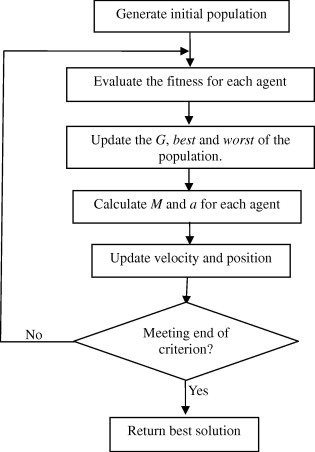
\includegraphics{Images/GSA.jpg}
            \end{center}
            \caption{The Gravitational Search Algorithm}
        \end{wrapfigure}

        The equation of motion of a physical system completely determines its dynamics, as such, it the goal of us as physicists (at least during the reading of the investigation) to find the sequence of positions that satisfy (i.e. solve) the equation of motion.  Analytically, the equation of motion is often a second-order differential equation, but an approximate solution can still be yielded.  There is a near infinite number of methods to approximating a solution to a differential equation (called \emph{numerical integrators}) using finite techniques, but equations \ref{eq:velocity} and \ref{eq:position} show how we use the so-called `symplectic Euler Method':

        \begin{align}
            \label{eq:velocity} v_n^i &= r_i v_{n-1}^i + a_{n - 1}^i \\
            \label{eq:position} x_n^i &= x_{n - 1}^i + v_n^i
        \end{align}

        where $x_n^i, v_n^i$ are the position and velocity, respectively, of mass $i$ at step $n$.

\clearpage
\newpage

    \subsection{The Discrete GSA}

        \begin{equation} \label{eq:force}
            F_{ij} = rand \times G \times \frac{M_j M_i}{NR_{ij}} R_{ij}
        \end{equation}

        \begin{equation} \label{eq:dml}
            a_{ij} = I_{ij} = \left\lceil \frac{F_{ij}}{M_i} \right\rceil = \left\lceil rand \times G \times \frac{M_j}{NR_{ij}} \times R_{ij} \right\rceil
        \end{equation}

        \begin{algorithm}
            \caption{The Discrete Gravitational Search Algorithm}
            \KwIn{$n$ as the size of input instance, $s$ as the number of searcher agents, $K_{\text{initial}}$ as the initial value of $K$, $G_{\text{initial}}$ as the initial value of the gravitational coefficient, and $G_{\text{end}}$ as the final value of the gravitational coefficient.}
            \tcp{initialization phase}
            $iteration \gets 0$\;
            Generate the initial population $P(iteration)$ of the solutions by greedy randomized algorithm\;
            Evaluate the fitnes for each agent of $P(iteration)$\;
            Calculate the gravitational mass for each agent of $P(iteration)$ by equation \ref{eq:mass}\;
            Generate the initial velocity $V(iteration)$ randomly\;
            \tcp{main phase}
            \While{stopping criteria is not satisfied}{
                \tcp{Dependent Movement Operator phase}
                Update $G, K$, and $Kbest$\;
                Calculate $I_{ij}$ for each agent $i$ and $j \in Kbest$ based on equation (\ref{eq:force})\;
                \For{i = 1 to s}{
                    $P_i(iteration + 1) \gets$ output of MTMNS algorithm execution with input parameters: $P_i$ as starting solutions, $K$ as the number of target solutions, $Kbest$ as target solution set, and $I_{ij}$ fo reach agent $j \in Kbest$ as movement lengths set
                }
                \tcp{Independent Movement Operator phase}
                \For{i = 1 to s}{
                    \tcp{$V_i$(iteration) is the previous movement length and $rand$ is a random number in $[0,1]$}
                    $IML \gets \lceil rand \times V_i \rceil$\;
                    $P_i(iteration + 1) \gets$ output of the modifed local search algorithm with input parameter: $P_i(iteration)$ as starting solution and $IML$ maximum movement length\;
                    Evaluate the fitness for each agent of $P(iteration + 1)$\;
                    Calculate the gravitaitonal mass for each agent of $P(iteration + 1)$ by equation (\ref{eq:mass})\;
                    $iteration \gets iteration + 1$
                }
            }
            \KwOut{Best solution found}
        \end{algorithm}
\newpage
\section{Results}

    \begin{table}[h!]
        \center{
        \begin{tabular}{|c||c|c|c|c|c|}
            \hline
            name & minimum & maximum & median & average & standard deviation \\
            \hline
            \hline
            burma14 & 3320.0 & 3340.0 & 3320.0 & 3330.0 & 5.85 \\
            \hline
            br17 & 39.0 & 41.0 & 39.0 & 39.2 & 0.504 \\
            \hline
            gr17 & 2080.0 & 2100.0 & 2080.0 & 2090.0 & 5.81 \\
            \hline
            gr21 & 2710.0 & 2970.0 & 2800.0 & 2770.0 & 69.9 \\
            \hline
            gr24 & 1270.0 & 1480.0 & 1350.0 & 1350.0 & 43.2 \\
            \hline
            fri26 & 955.0 & 1080.0 & 989.0 & 994.0 & 33.9 \\
            \hline
            bayg29 & 1630.0 & 1840.0 & 1710.0 & 1720.0 & 50.5 \\
            \hline
            bays29 & 2090.0 & 2330.0 & 2170.0 & 2180.0 & 68.7 \\
            \hline
            ftv33 & 1430.0 & 1670.0 & 1560.0 & 1560.0 & 57.1 \\
            \hline
            ftv35 & 1610.0 & 1920.0 & 1760.0 & 1750.0 & 73.9 \\
            \hline
            ftv38 & 1620.0 & 1940.0 & 1850.0 & 1850.0 & 72.6 \\
            \hline
            dantzig42 & 771.0 & 906.0 & 838.0 & 838.0 & 36.9 \\
            \hline
            swiss42 & 1390.0 & 1640.0 & 1510.0 & 1510.0 & 59.8 \\
            \hline
            p43 & 5650.0 & 5710.0 & 5680.0 & 5680.0 & 14.3 \\
            \hline
            ftv44 & 1890.0 & 2250.0 & 2020.0 & 2040.0 & 91.7 \\
            \hline
            ftv47 & 2120.0 & 2470.0 & 2300.0 & 2300.0 & 78.7 \\
            \hline
            att48 & 11300.0 & 14200.0 & 12500.0 & 12600.0 & 796.0 \\
            \hline
            gr48 & 5600.0 & 6770.0 & 6070.0 & 6050.0 & 242.0 \\
            \hline
            hk48 & 12400.0 & 14500.0 & 13400.0 & 13400.0 & 539.0 \\
            \hline
            ry48p & 15400.0 & 18900.0 & 17200.0 & 17300.0 & 753.0 \\
            \hline
            berlin52 & 8450.0 & 10000.0 & 9060.0 & 9080.0 & 353.0 \\
            \hline
            ft53 & 8350.0 & 10200.0 & 9130.0 & 9180.0 & 400.0 \\
            \hline
            ftv55 & 2020.0 & 2460.0 & 2240.0 & 2240.0 & 115.0 \\
            \hline
            brazil58 & 29400.0 & 35000.0 & 31600.0 & 31800.0 & 1250.0 \\
            \hline
            ftv64 & 2480.0 & 2920.0 & 2680.0 & 2680.0 & 124.0 \\
            \hline
            ft70 & 41900.0 & 44300.0 & 43200.0 & 43200.0 & 521.0 \\
            \hline
            ftv70 & 2630.0 & 3140.0 & 2900.0 & 2900.0 & 113.0 \\
            \hline
            st70 & 853.0 & 995.0 & 917.0 & 921.0 & 42.2 \\
            \hline
            eil76 & 634.0 & 728.0 & 679.0 & 681.0 & 22.1 \\
            \hline
            pr76 & 133000.0 & 155000.0 & 146000.0 & 145000.0 & 6310.0 \\
            \hline
            gr96 & 72200.0 & 91100.0 & 82000.0 & 81600.0 & 4730.0 \\
            \hline
            rat99 & 1480.0 & 1860.0 & 1750.0 & 1740.0 & 83.2 \\
            \hline
            kroA100 & 31500.0 & 38100.0 & 34600.0 & 34600.0 & 1840.0 \\
            \hline
            kroB100 & 31000.0 & 37100.0 & 34800.0 & 34600.0 & 1580.0 \\
            \hline
            kroC100 & 30900.0 & 37700.0 & 34300.0 & 34400.0 & 1840.0 \\
            \hline
            kroD100 & 29700.0 & 38600.0 & 33800.0 & 34200.0 & 2210.0 \\
            \hline
            kroE100 & 32500.0 & 40800.0 & 35100.0 & 35400.0 & 2000.0 \\
            \hline
            rd100 & 11000.0 & 12900.0 & 12200.0 & 12200.0 & 461.0 \\
            \hline
            eil101 & 773.0 & 928.0 & 859.0 & 853.0 & 35.1 \\
            \hline
        \end{tabular}
        }
        \caption{Statistical summary of results for the Discrete Gravitaitonal Search on problems up to 100 cities}
    \end{table}

    \begin{table}[h!]
        \center{
        \begin{tabular}{|c||c|c|c|c|c|}
            \hline
            name & minimum & maximum & median & average & standard deviation \\
            \hline
            \hline
            lin105 & 21100.0 & 26200.0 & 23700.0 & 23800.0 & 1250.0 \\
            pr107 & 78500.0 & 142000.0 & 115000.0 & 114000.0 & 12700.0 \\
            gr120 & 9630.0 & 11600.0 & 10800.0 & 10800.0 & 496.0 \\ 
            kro124p & 50300.0 & 55400.0 & 53000.0 & 53000.0 & 1420.0 \\
            pr124 & 88200.0 & 136000.0 & 123000.0 & 120000.0 & 11600.0 \\
            bier127 & 146000.0 & 176000.0 & 163000.0 & 163000.0 & 5550.0 \\
            ch130 & 9280.0 & 10800.0 & 9830.0 & 9930.0 & 383.0 \\
            pr136 & 152000.0 & 180000.0 & 165000.0 & 164000.0 & 7120.0 \\
            gr137 & 106000.0 & 126000.0 & 118000.0 & 118000.0 & 5940.0 \\
            pr144 & 136000.0 & 175000.0 & 158000.0 & 157000.0 & 9750.0 \\
            ch150 & 9800.0 & 11700.0 & 10800.0 & 10700.0 & 390.0 \\
            kroA150 & 42400.0 & 54200.0 & 47800.0 & 47700.0 & 2680.0 \\
            kroB150 & 43400.0 & 53000.0 & 47300.0 & 47600.0 & 2180.0 \\
            pr152 & 180000.0 & 238000.0 & 203000.0 & 204000.0 & 13100.0 \\
            u159 & 68200.0 & 89700.0 & 80100.0 & 79600.0 & 5000.0 \\
            ftv170 & 5670.0 & 6740.0 & 6330.0 & 6280.0 & 277.0 \\
            si175 & 25700.0 & 26800.0 & 26300.0 & 26200.0 & 265.0 \\
            brg180 & 3680.0 & 4230.0 & 4000.0 & 3980.0 & 154.0 \\
            rat195 & 3680.0 & 4310.0 & 3960.0 & 3960.0 & 172.0 \\
            d198 & 25800.0 & 35800.0 & 32100.0 & 31700.0 & 2430.0 \\
            kroA200 & 51900.0 & 64500.0 & 58900.0 & 58700.0 & 2780.0 \\
            kroB200 & 54000.0 & 62200.0 & 58600.0 & 58400.0 & 2320.0 \\
            \hline
        \end{tabular}
        }
        \caption{Statistical summary of results for the Discrete Gravitaitonal Search on problems up to between 101 and 200 cities}
    \end{table}
\section{Conclusion}

\pagebreak
\nocite*{}
\bibliography{references}


\end{document}
